% !TEX program = xelatex
\documentclass[9pt, aspectratio=169]{beamer}
\usetheme{metropolis}
\usefonttheme{professionalfonts}

% --- Modern Font Setup ---
\usepackage[T1]{fontenc}
\usepackage{FiraSans}  % Modern, elegant sans-serif font family
\usepackage[scaled=0.95]{FiraMono}  % Matching monospace font

% Lighter, more refined font weights
\renewcommand{\seriesdefault}{l}  % Light weight as default
\renewcommand{\bfseries}{\fontseries{sb}\selectfont}  % Semi-bold instead of bold

% Custom font sizing - more refined
\setbeamerfont{title}{size=\Large, series=\fontseries{m}\selectfont}
\setbeamerfont{subtitle}{size=\normalsize, series=\fontseries{l}\selectfont}
\setbeamerfont{author}{size=\small, series=\fontseries{l}\selectfont}
\setbeamerfont{date}{size=\small, series=\fontseries{l}\selectfont}
\setbeamerfont{frametitle}{size=\normalsize, series=\fontseries{m}\selectfont}
\setbeamerfont{framesubtitle}{size=\footnotesize, series=\fontseries{l}\selectfont}
\setbeamerfont{block title}{size=\normalsize, series=\fontseries{m}\selectfont}
\setbeamerfont{block body}{size=\small}
\setbeamerfont{itemize/enumerate body}{size=\small}
\setbeamerfont{itemize/enumerate subbody}{size=\footnotesize}
\setbeamerfont{section in toc}{size=\normalsize, series=\fontseries{m}\selectfont}
\setbeamerfont{section title}{size=\Large, series=\fontseries{m}\selectfont}

% --- Color Definitions ---
% Primary Theme Colors
\definecolor{PrimaryColor}{RGB}{33,52,72}         % Deep navy
\definecolor{SecondaryColor}{RGB}{84,119,146}     % Desaturated blue-gray
\definecolor{AccentColor}{RGB}{100,156,165}       % Soft steel blue
\definecolor{black}{RGB}{0,0,0}
\definecolor{BackgroundColor}{RGB}{245,247,250}   % Very light cool gray/blue-tinted white
\definecolor{TextColor}{RGB}{40,55,70}            % Darker, cool-toned charcoal
\definecolor{LightGray}{RGB}{220,225,230}         % Soft, cool light gray
\definecolor{DarkGray}{RGB}{70,90,105}            % Cool-toned dark gray

% --- Theme Customization ---
\setbeamercolor{background canvas}{bg=BackgroundColor}
\setbeamercolor{normal text}{fg=TextColor}
\setbeamercolor{frametitle}{bg=PrimaryColor, fg=white}
\setbeamercolor{section in toc}{fg=PrimaryColor}
\setbeamercolor{block title}{bg=PrimaryColor!80, fg=white}
\setbeamercolor{block body}{bg=PrimaryColor!10}
\setbeamercolor{alerted text}{fg=AccentColor}
\setbeamercolor{itemize item}{fg=PrimaryColor}
\setbeamercolor{itemize subitem}{fg=SecondaryColor}

% Progress bar
\setbeamercolor{progress bar}{fg=AccentColor, bg=LightGray}

% --- Packages ---
\usepackage[utf8]{inputenc}
\usepackage{url}
\usepackage{booktabs}
\usepackage{amsmath, amssymb, amsfonts}
\usepackage{fontawesome5}
\usepackage{pifont}
\usepackage[most]{tcolorbox}
\tcbuselibrary{skins, listings}
\usepackage{colortbl}
\usepackage{array}
\usepackage{adjustbox}
\usepackage{ragged2e}

% --- Packages for plotting discrete and continuous signals and spectrums ---
\usepackage{tikz}
\usepackage{circuitikz} % Useful for signal processing block diagrams
\usepackage{pgfplots}
\usepackage{graphicx}
\usepackage{caption}
\usepackage{subcaption}

\usetikzlibrary{shapes.callouts, positioning, arrows.meta, shapes.geometric, shadows, calc, patterns, backgrounds, shadings, fit, chains, decorations.pathreplacing, intersections}
\usepgfplotslibrary{fillbetween}
\usepgfplotslibrary{polar}
\pgfplotsset{compat=1.18}
\pgfplotsset{
    plot coordinates/math parser=false,
    signal/.style={thick, color=PrimaryColor},
    spectrum/.style={thick, color=AccentColor},
    discrete/.style={ycomb, mark=*, mark options={fill=white, draw=PrimaryColor}, color=PrimaryColor, thick},
}

% --- Custom Commands ---
\newcommand{\cmark}{\textcolor{PrimaryColor}{\ding{51}}}
\newcommand{\xmark}{\textcolor{AccentColor}{\ding{55}}}
\newcommand{\highlight}[1]{\textcolor{PrimaryColor}{\textbf{#1}}}

% --- Custom tcolorbox environments ---
\newtcolorbox{conceptbox}[1]{
    colback=PrimaryColor!10,
    colframe=PrimaryColor,
    title=#1,
    fonttitle=\small\bfseries,
    fontupper=\small,
    rounded corners
}

\newtcolorbox{insightbox}[1]{
    colback=AccentColor!10,
    colframe=AccentColor,
    title=#1,
    fonttitle=\small\bfseries,
    fontupper=\small,
    rounded corners
}

\newtcolorbox{algorithmbox}[1]{
    colback=SecondaryColor!10,
    colframe=SecondaryColor,
    title=#1,
    fonttitle=\small\bfseries,
    fontupper=\small,
    rounded corners
}

\newtcblisting{codelistingbox}[2][]{
    colback=SecondaryColor!10,
    colframe=SecondaryColor,
    title=#2,
    fonttitle=\small\bfseries,
    rounded corners,
    listing only,
    listing options={
            language=#1,
            basicstyle=\ttfamily\footnotesize,
            keywordstyle=\color{PrimaryColor}\bfseries,
            commentstyle=\color{SecondaryColor}\itshape,
            stringstyle=\color{AccentColor},
            numbers=left,
            numberstyle=\tiny\color{DarkGray},
            stepnumber=1,
            showstringspaces=false,
            tabsize=4
        }
}


\subtitle{Signals and Linear Systems}
\date{}
\author{Ashrafur Rahman\\Lecturer, CSE, BUET}
\institute{ashrafur@cse.buet.ac.bd}


\title{Recap on DFT}

\begin{document}

\maketitle

\begin{frame}{Outline}
    \begin{itemize}
        \item \textbf{Review:} CTFS, DTFS, and the DFT
        \item \textbf{Aperiodic Signals:} The DTFT and its relationship to the DFT
        \item \textbf{Zero-Padding:} Increasing frequency-domain resolution
        \item \textbf{The Need for Speed:} Naive DFT complexity
        \item \textbf{Fast Fourier Transform (FFT):}
              \begin{itemize}
                  \item Radix-2 Decimation-in-Time (DIT)
                  \item Radix-2 Decimation-in-Frequency (DIF)
              \end{itemize}
        \item \textbf{Conclusion:} FFT Complexity Analysis
    \end{itemize}
\end{frame}

\begin{frame}{Recap of CTFS}
    \begin{minipage}{0.5\textwidth}
        \begin{itemize}
            \item Let's start with a Continuous-time periodic signal $x(t)$ with period $T_0$:
                  \begin{equation*}
                      x(t+T_0)=x(t), \quad \omega_0 \triangleq \frac{2\pi}{T_0}.
                  \end{equation*}
            \item We have learnt the Continuous Time Fourier Series (CTFS) representation is:
        \end{itemize}
        \begin{conceptbox}{CTFS Pair}
            \vspace{-0.4cm}
            \begin{align*}
                x(t) & = \sum c_k e^{jk\omega_0 t}                            \\
                c_k  & = \frac{1}{T_0}\int_{T_0} \!\! x(t)e^{-jk\omega_0 t}dt
            \end{align*}
        \end{conceptbox}
    \end{minipage}
    \hfill
    \begin{minipage}{0.48\textwidth}
        \begin{center}
            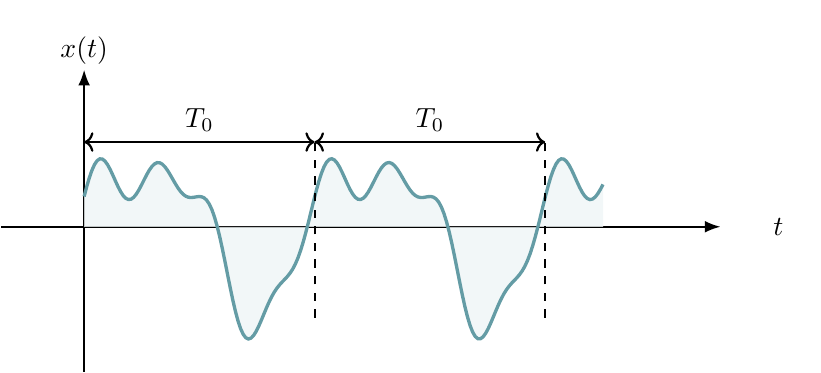
\begin{tikzpicture}[scale=0.8]
                \begin{axis}[
                    width=\textwidth, height=5.5cm,
                    axis lines=middle, axis line style={shorten >=-10pt, shorten <=-10pt, -{Latex[length=2mm]}, thick},
                    xmin=0, xmax=3.2, ymin=-1.6, ymax=1.8,
                    xtick=\empty, ytick=\empty,
                    xlabel={$t$}, ylabel={$x(t)$},
                    xlabel style={at={(axis cs:4.1,0)}, anchor=east},
                    ylabel style={at={(axis cs:0,3.3)}, anchor=north},
                    clip=false, enlargelimits=0.1,
                    declare function={sig(\t) = 1.2*sin(deg(1.5*pi*\t)) + 0.5*cos(deg(3*pi*\t)) + 0.3*sin(deg(6*pi*\t));}
                    ]
                    % Custom signal
                    \addplot[name path=f, samples=200, domain=0:3.0, very thick, AccentColor] {sig(x)};
                    \path[name path=axis] (axis cs:0,0) -- (axis cs:3.0,0);
                    \addplot [AccentColor!10, opacity=0.8] fill between [of=f and axis];

                    \addplot[dashed, thick] coordinates {(1.333,-1.5) (1.333,1.5)};
                    \addplot[dashed, thick] coordinates {(2.666,-1.5) (2.666,1.5)};
                    \draw[<->, thick] (axis cs:0,1.4) -- node[midway, above] {$T_0$} (axis cs:1.333,1.4);
                    \draw[<->, thick] (axis cs:1.333,1.4) -- node[midway, above] {$T_0$} (axis cs:2.666,1.4);
                \end{axis}
            \end{tikzpicture}
        \end{center}
    \end{minipage}
\end{frame}

\begin{frame}{Uniform Sampling}
    We are now interested in a representation for discrete signals. We can sample $x(t)$ to get a discrete signal $x[n]$.

    \begin{minipage}{0.48\textwidth}
        \begin{itemize}
            \item Sample $x(t)$ uniformly with sampling period $T_s$.
            \item Assume $T_0$ is captured by $N$ samples:
                  \begin{equation*}
                      T_0 = N T_s \quad (N \in \mathbb{Z}^+).
                  \end{equation*}
            \item The purely discrete sequence $x[n]$ is defined as:
                  \begin{equation*}
                      x[n] \triangleq x(nT_s), \quad n \in \mathbb{Z}.
                  \end{equation*}
            \item Thus $x[n]$ is inherently \textbf{$N$-periodic}:
                  \begin{equation*}
                      x[n+N]=x[n].
                  \end{equation*}
        \end{itemize}
    \end{minipage}
    \hfill
    \begin{minipage}{0.48\textwidth}
        \begin{center}
            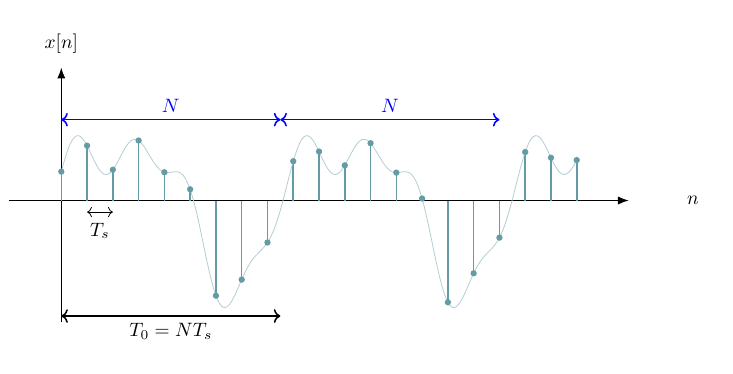
\begin{tikzpicture}[scale=0.7]
                \begin{axis}[
                    width=\textwidth, height=5.5cm,
                    axis lines=middle, axis line style={shorten >=-10pt, shorten <=-10pt, -{Latex[length=2mm]}, thick},
                    xmin=-0.5, xmax=40.5, ymin=-1.6, ymax=1.8,
                    xtick=\empty,
                    ytick=\empty,
                    xlabel={$n$}, ylabel={$x[n]$},
                    xlabel style={at={(axis cs:50,0)}, anchor=east},
                    ylabel style={at={(axis cs:0,3)}, anchor=north},
                    clip=false, enlargelimits=0.05,
                    declare function={sig(\t) = 1.2*sin(deg(1.5*pi*\t)) + 0.5*cos(deg(3*pi*\t)) + 0.3*sin(deg(6*pi*\t));}
                    ]
                    \addplot[ycomb, mark=*, mark size=1.2pt, thick, domain=0:40, samples=21, color=AccentColor] {sig(x*0.075)};
                    \addplot[name path=f, samples=200, domain=0:40, thin, AccentColor!50] {sig(x*0.075)};
                    \draw[<->, thin] (axis cs:2,-0.2) -- node[midway, below, yshift=-2pt] {$T_s$} (axis cs:4,-0.2);
                    \draw[<->, thick] (axis cs:0,-2) -- node[midway, below] {$T_0=NT_s$} (axis cs:17,-2);
                    \draw[<->, thick, blue] (axis cs:0,1.4) -- node[midway, above] {$N$} (axis cs:17,1.4);
                    \draw[<->, thick, blue] (axis cs:17,1.4) -- node[midway, above] {$N$} (axis cs:34,1.4);
                \end{axis}
            \end{tikzpicture}
        \end{center}
    \end{minipage}
\end{frame}

\begin{frame}{Impulse-Train Representation of Sampling}
    \begin{itemize}
        \item We can represent the sampled signal mathematically using an impulse train (aka Dirac comb).
        \item Multiplying the continuous signal $x(t)$ with the impulse train $p(t)$ gives us the sampled signal $x_p(t)$.
        \item Each sample $x[n]$ is weighted by a Dirac delta function at time $nT_s$.
    \end{itemize}

    \begin{minipage}{0.48\textwidth}
        \centering
        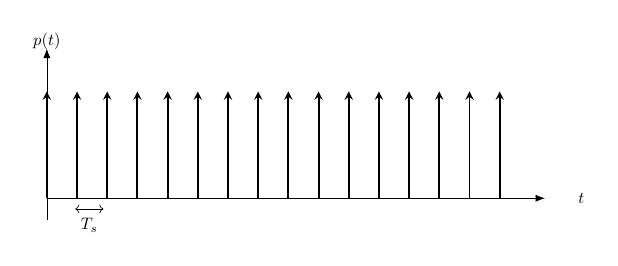
\begin{tikzpicture}[scale=0.6]
            \begin{axis}[
                width=\linewidth, height=5.2cm,
                axis lines=middle, axis line style={-{Latex[length=2mm]}},
                xmin=0, xmax=2.2, ymin=-0.2, ymax=1.4,
                xtick=\empty, ytick=\empty,
                xlabel={$t$}, ylabel={$p(t)$},
                xlabel style={at={(axis cs:2.4,0)}, anchor=east},
                ylabel style={at={(axis cs:0,1.6)}, anchor=north},
                clip=false
                ]
                % Draw impulse train with arrows
                \addplot[quiver={u=0,v=1}, -{stealth[length=2.5mm, width=2.5mm]}, very thick, domain=0:2.0, samples=16, color=black] {0};
                \draw[<->] (axis cs:0.125,-0.1) -- node[midway, below, yshift=-2pt] {$T_s$} (axis cs:0.25,-0.1);
            \end{axis}
        \end{tikzpicture}
        \vspace{0.1cm}

        Impulse train $p(t) = \sum \delta(t-nT_s)$.
    \end{minipage}
    \hfill
    \begin{minipage}{0.48\textwidth}
        \centering
        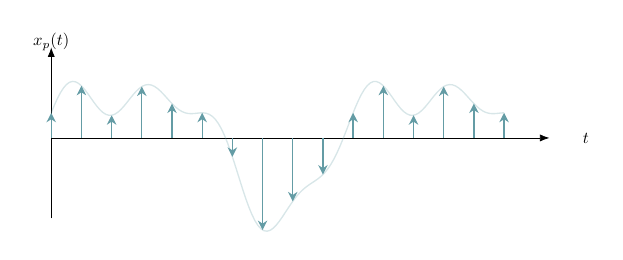
\begin{tikzpicture}[scale=0.6]
            \begin{axis}[
                width=\linewidth, height=5.2cm,
                axis lines=middle, axis line style={-{Latex[length=2mm]}},
                xmin=0, xmax=2.2, ymin=-1.6, ymax=1.8,
                xtick=\empty, ytick=\empty,
                xlabel={$t$}, ylabel={$x_p(t)$},
                xlabel style={at={(axis cs:2.4,0)}, anchor=east},
                ylabel style={at={(axis cs:0,2.2)}, anchor=north},
                clip=false,
                declare function={sig(\t) = 1.2*sin(deg(1.5*pi*\t)) + 0.5*cos(deg(3*pi*\t)) + 0.3*sin(deg(6*pi*\t));}
                ]
                \addplot[samples=150,domain=0:2.0,thick,opacity=0.25, AccentColor] {sig(x)};
                \addplot[quiver={u=0,v=sig(x)}, -{Stealth[length=2mm, width=2mm]}, thick, domain=0:2.0, samples=16, color=AccentColor] {0};
            \end{axis}
        \end{tikzpicture}
        \vspace{0.1cm}

        Sampled signal $x_p(t) = x(t)p(t)$.
    \end{minipage}

    \vspace{0.2cm}
    \begin{align*}
        x_p(t) = \sum_{n=-\infty}^{\infty} x(nT_s)\,\delta(t-nT_s) = \sum_{n=-\infty}^{\infty} x[n]\,\delta(t-nT_s).
    \end{align*}
\end{frame}

\begin{frame}{CTFS of the Sampled Signal}
    Now let us find the CTFS of the sampled signal $x_p(t)$.
    \begin{itemize}
        \item Let $c_k$ denote the CTFS coefficients of the $T_0$-periodic sampled signal $x_p(t)$:
              \begin{equation*}
                  x_p(t) = \sum_{k=-\infty}^{\infty} c_k e^{jk\omega_0 t}, \qquad c_k = \frac{1}{T_0}\int_{T_0} x_p(t)\,e^{-jk\omega_0 t}\,dt.
              \end{equation*}
        \item Substitute $x_p(t) = \sum_{n=-\infty}^{\infty} x[n]\delta(t-nT_s)$ into the analysis equation:
              \begin{align*}
                  c_k & = \frac{1}{T_0}\int_{t_0}^{ t_0+T_0} \left(\sum_{n=-\infty}^{\infty} x[n]\delta(t-nT_s)\right)e^{-jk\omega_0 t}\,dt \\
                      & = \frac{1}{T_0}\sum_{n=0}^{N-1} x[n] \int_{t_0}^{t_0+T_0}\delta(t-nT_s)e^{-jk\omega_0 t}\,dt                        \\
                      & = \frac{1}{T_0}\sum_{n=0}^{N-1} x[n]\,e^{-jk\omega_0 nT_s}                                                          \\
                      & = \frac{1}{T_0}\sum_{n=0}^{N-1} x[n]\,e^{-j\frac{2\pi}{N}kn}.
              \end{align*}
    \end{itemize}
    {\footnotesize We can take $t_0 = -\frac{T_s}{2}$, so $\delta(t-nT_s)$ is non-zero in $[t_0, t_0+T_0]$ only for $n=0,1,2,\dots,N-1$.}
\end{frame}

\begin{frame}{Periodicity of $c_k$}
    \begin{minipage}{0.48\textwidth}
        \begin{itemize}
            \item Examine the exponent in $c_k$:
                  \begin{align*}
                      c_{k+N} & = \frac{1}{T_0}\sum_{n=0}^{N-1} x[n]e^{-j\frac{2\pi}{N}(k+N)n} \\
                              & = c_k \underbrace{e^{-j2\pi n}}_{=1} = c_k
                  \end{align*}
            \item The contiguous frequency coefficients are $N$-periodic!
            \item \textbf{Only $N$ unique frequency values} exist before the spectrum repeats.
            \item Leads to the $N$-point Discrete Fourier Transform.
        \end{itemize}
    \end{minipage}
    \hfill
    \begin{minipage}{0.48\textwidth}
        \begin{center}
            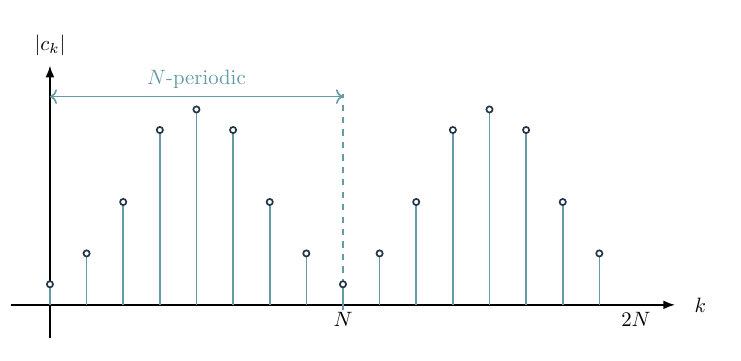
\begin{tikzpicture}[scale=0.75]
                \begin{axis}[
                    width=\textwidth, height=5.5cm,
                    axis lines=middle, axis line style={shorten >=-10pt, shorten <=-10pt, -{Latex[length=2mm]}, thick},
                    xmin=-0.5, xmax=16.5, ymin=-0.5, ymax=8.5,
                    xtick=\empty, ytick=\empty,
                    xlabel={$k$}, ylabel={$|c_k|$},
                    xlabel style={xshift=1cm,anchor=east},
                    ylabel style={yshift=1cm,anchor=north},
                    clip=false
                    ]
                    \addplot+[discrete, spectrum, mark=*, mark size=1.5pt] coordinates {
                            (0,0.8) (1,2.0) (2,4.0) (3,6.8) (4,7.6) (5,6.8) (6,4.0) (7,2.0)
                            (8,0.8) (9,2.0) (10,4.0) (11,6.8) (12,7.6) (13,6.8) (14,4.0) (15,2.0)
                        };
                    \node[anchor=north] at (axis cs:8,0) {$N$};
                    \node[anchor=north] at (axis cs:16,0) {$2N$};
                    \draw[dashed, AccentColor, thick] (axis cs:8,-0.2) -- (axis cs:8,8.2);
                    \draw[<->, AccentColor, thick] (axis cs:0,8.1) -- node[above, AccentColor] {$N$-periodic} (axis cs:8,8.1);
                \end{axis}
            \end{tikzpicture}
        \end{center}
    \end{minipage}
\end{frame}

\begin{frame}{Definition of the $N$-point DFT}
    \begin{itemize}
        \item The $N$-point \textbf{discrete Fourier transform (DFT)} of a length-$N$ sequence $\{x[n]\}_{n=0}^{N-1}$ is defined simply as a scaled version of one period of the unique $c_k$ components:
    \end{itemize}

    \vspace{0.2cm}
    \begin{conceptbox}{Discrete Fourier Transform (DFT)}
        \vspace{-0.2cm}
        \begin{equation*}
            X[k] \triangleq \sum_{n=0}^{N-1} x[n]\,e^{-j\frac{2\pi}{N}kn}, \qquad k=0,1,\dots,N-1
        \end{equation*}
    \end{conceptbox}

    \begin{itemize}
        \item Thus, the relationship is $c_k = \frac{1}{T_0}X[k]$.
    \end{itemize}
\end{frame}

\begin{frame}{Recovering the Discrete Sequence}
    \begin{itemize}
        \item<1-> We cannot simply use the CTFS synthesis equation to recover our signal:
              \begin{equation*}
                  x(t) = \sum_{k=-\infty}^{\infty} c_k e^{jk\omega_0 t}
              \end{equation*}
        \item<1-> This equation evaluates to the continuous-time impulse train $x_p(t)$, not the purely discrete sequence $x[n]$ which we desire.
        \item<2-> However, there is a general pattern in transforms from our experience:
              \begin{itemize}
                  \item \textbf{Forward Transform} (Analysis) usually uses $e^{-j\dots}$ (e.g., $e^{-jk\omega_0 t}$)
                  \item \textbf{Inverse Transform} (Synthesis) usually uses $e^{+j\dots}$ (e.g., $e^{+jk\omega_0 t}$)
              \end{itemize}
        \item<2-> Let's apply this intuitive pattern to derive an explicit recovery formula for $x[n]$ using $e^{+j\dots}$.
    \end{itemize}
\end{frame}

\begin{frame}{Deriving the Inverse DFT (1/2)}
    \begin{itemize}
        \item Multiply both sides of the DFT by $e^{j\frac{2\pi}{N}kn}$ and sum over $k$:
              \begin{align*}
                  \sum_{k=0}^{N-1} X[k] e^{j\frac{2\pi}{N}kn} & = \sum_{k=0}^{N-1} \left( \sum_{m=0}^{N-1} x[m] e^{-j\frac{2\pi}{N}km} \right) e^{j\frac{2\pi}{N}kn} \\
                                                              & = \sum_{m=0}^{N-1} x[m] \left( \sum_{k=0}^{N-1} e^{j\frac{2\pi}{N}k(n-m)} \right)
              \end{align*}
        \item Evaluate the inner summation using the geometric series sum formula. For $n \neq m$:
              \begin{equation*}
                  \sum_{k=0}^{N-1} \left( e^{j\frac{2\pi}{N}(n-m)} \right)^k = \frac{1 - e^{j2\pi(n-m)}}{1 - e^{j\frac{2\pi}{N}(n-m)}} = \frac{1 - 1}{1 - e^{j\frac{2\pi}{N}(n-m)}} = 0
              \end{equation*}
    \end{itemize}
\end{frame}

\begin{frame}{Deriving the Inverse DFT (2/2)}
    \begin{itemize}
        \item And for $n = m$, the summation simply evaluates to:
              \begin{equation*}
                  \sum_{k=0}^{N-1} e^0 = N \implies \sum_{k=0}^{N-1} e^{j\frac{2\pi}{N}k(n-m)} = \begin{cases} N & n = m \\ 0 & n \neq m \end{cases}
              \end{equation*}
        \item Applying this to the previous equation, all terms in the outer sum become zero except when $m=n$:
              \begin{equation*}
                  \sum_{k=0}^{N-1} X[k] e^{j\frac{2\pi}{N}kn} = x[n] \cdot N
              \end{equation*}
        \item Rearranging for $x[n]$ gives the \textbf{Inverse DFT (IDFT)}:
    \end{itemize}
    \vspace{0.1cm}
    \begin{conceptbox}{Inverse Discrete Fourier Transform (IDFT)}
        \vspace{-0.2cm}
        \begin{equation*}
            x[n] = \frac{1}{N}\sum_{k=0}^{N-1} X[k]\,e^{j\frac{2\pi}{N}kn}, \qquad n=0,1,\dots,N-1
        \end{equation*}
    \end{conceptbox}

\end{frame}\begin{frame}{Recap: The DFT for Periodic Signals}
    \begin{minipage}{0.48\textwidth}
        \begin{itemize}
            \item We started with a continuous-time periodic signal $x(t)$.
            \item Sampling it yielded a \textbf{periodic discrete sequence} $x[n]$ with period $N$.
            \item Its frequency representation $c_k$ is uniquely defined by exactly $N$ contiguous components.
            \item Ultimately, the \textbf{DFT} transforms exactly $N$ points of $x[n]$ into $N$ unique frequency coefficients $X[k]$.
            \item The \textbf{IDFT} perfectly reconstructs those $N$ points in time from these $N$ frequency values.
        \end{itemize}
    \end{minipage}
    \hfill
    \begin{minipage}{0.48\textwidth}
        \begin{center}
            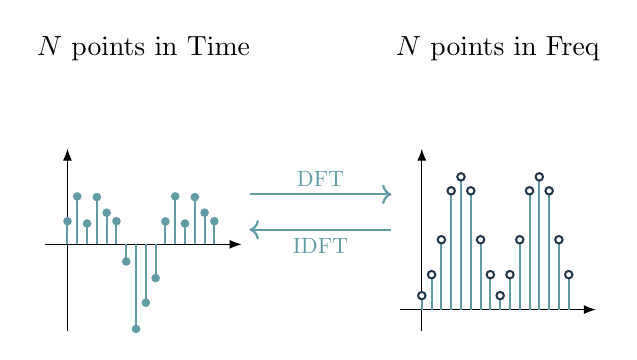
\begin{tikzpicture}[scale=0.9]
                \node at (0,3.3) {$N$ points in Time};
                \draw[->, thick, AccentColor] (1.5,1.25) -- node[above, scale=0.8] {DFT} (3.5,1.25);
                \draw[<-, thick, AccentColor] (1.5,0.75) -- node[below, scale=0.8] {IDFT} (3.5,0.75);
                \node at (5,3.3) {$N$ points in Freq};

                \begin{axis}[
                    at={(0,-0.5cm)}, anchor=south,
                    width=4cm, height=3.8cm,
                    axis lines=middle, axis line style={shorten >=-5pt, shorten <=-5pt, -{Latex}},
                    xmin=-1, xmax=16.5, ymin=-1.6, ymax=1.8,
                    xtick=\empty, ytick=\empty, clip=false,
                    declare function={sig(\t) = 1.2*sin(deg(1.5*pi*\t)) + 0.5*cos(deg(3*pi*\t)) + 0.3*sin(deg(6*pi*\t));}
                    ]
                    \addplot[ycomb, mark=*, AccentColor, thick, samples=16, domain=0:15, mark size=1.3pt] {sig(x*0.1333)};
                \end{axis}
                \begin{axis}[
                    at={(5cm,-0.5cm)}, anchor=south,
                    width=4cm, height=3.8cm,
                    axis lines=middle, axis line style={shorten >=-5pt, shorten <=-5pt, -{Latex}},
                    xmin=-1, xmax=16.5, ymin=-0.5, ymax=8.5,
                    xtick=\empty, ytick=\empty, clip=false
                    ]
                    \addplot+[discrete, spectrum, mark=*, AccentColor, thick, mark size=1.5pt] coordinates {
                            (0,0.8) (1,2.0) (2,4.0) (3,6.8) (4,7.6) (5,6.8) (6,4.0) (7,2.0)
                            (8,0.8) (9,2.0) (10,4.0) (11,6.8) (12,7.6) (13,6.8) (14,4.0) (15,2.0)
                        };
                \end{axis}
            \end{tikzpicture}
        \end{center}
    \end{minipage}
\end{frame}

\begin{frame}{What about Aperiodic Signals?}
    But does DFT only apply to periodic signals? What if the signal is aperiodic?
    \begin{itemize}
        \item Let's consider an aperiodic signal $x(t)$ restricted to a finite interval $T_0$.
        \item Uniformly sampling this yields a finite-length sequence $x[n]$ that is nonzero only for $0 \le n \le N-1$.
        \item Using the pulse train sampling method, we can represent the sampled signal as:
              \begin{equation*}
                  x_p(t) = x(t)p(t) = \sum_{n=-\infty}^{\infty} x[n] \delta(t - nT)  = \sum_{n=0}^{N-1} x[n] \delta(t - nT)
              \end{equation*}
    \end{itemize}
    \vspace{0.3cm}
    \begin{center}
        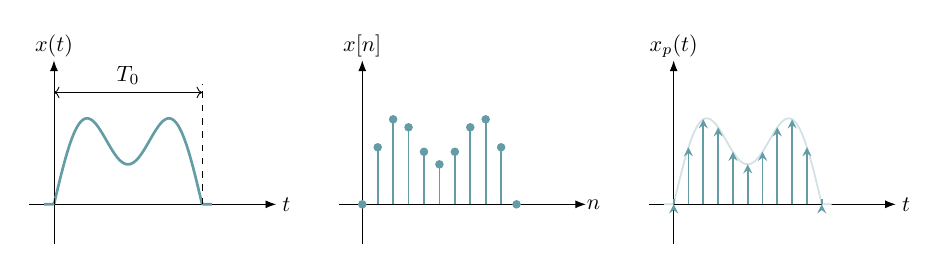
\begin{tikzpicture}[scale=0.8]
            \begin{axis}[
                name=ax1,
                width=5.5cm, height=4.5cm,
                axis lines=middle, axis line style={-{Latex}},
                xmin=-0.5, xmax=4.5, ymin=-0.5, ymax=1.8,
                xtick=\empty, ytick=\empty,
                xlabel={$t$}, ylabel={$x(t)$}, clip=false,
                ylabel style={yshift=15pt, anchor=north},
                xlabel style={xshift=10pt, anchor=east},
                declare function={sig(\t) = (\t>=0 && \t<=3) ? (sin(deg(pi*\t/3)) + 0.5*sin(deg(pi*\t))) : 0;}
                ]
                \addplot[samples=100, domain=-0.2:3.2, very thick, AccentColor] {sig(x)};
                \draw[dashed] (axis cs:0,0) -- (axis cs:0,1.5);
                \draw[dashed] (axis cs:3,0) -- (axis cs:3,1.5);
                \draw[<->] (axis cs:0,1.4) -- node[above] {$T_0$} (axis cs:3,1.4);
            \end{axis}

            \begin{axis}[
                name=ax2, at={(ax1.east)}, anchor=west, xshift=1cm,
                width=5.5cm, height=4.5cm,
                axis lines=middle, axis line style={-{Latex}},
                xmin=-1.5, xmax=14.5, ymin=-0.5, ymax=1.8,
                xtick=\empty, ytick=\empty,
                xlabel={$n$}, ylabel={$x[n]$}, clip=false,
                ylabel style={yshift=15pt, anchor=north},
                xlabel style={xshift=10pt, anchor=east},
                declare function={sig(\t) = (\t>=0 && \t<=10) ? (sin(deg(pi*\t/10)) + 0.5*sin(deg(3*pi*\t/10))) : 0;}
                ]
                \addplot[ycomb, mark=*, mark size=1.5pt, thick, AccentColor, samples=11, domain=0:10] {sig(x)};
            \end{axis}

            \begin{axis}[
                name=ax3, at={(ax2.east)}, anchor=west, xshift=1cm,
                width=5.5cm, height=4.5cm,
                axis lines=middle, axis line style={-{Latex}},
                xmin=-0.5, xmax=4.5, ymin=-0.5, ymax=1.8,
                xtick=\empty, ytick=\empty,
                ylabel style={yshift=15pt, anchor=north},
                xlabel style={xshift=10pt, anchor=east},
                xlabel={$t$}, ylabel={$x_p(t)$}, clip=false,
                declare function={sig(\t) = (\t>=0 && \t<=3) ? (sin(deg(pi*\t/3)) + 0.5*sin(deg(pi*\t))) : 0;}
                ]
                \addplot[samples=100, domain=-0.2:3.2, thick, AccentColor!30] {sig(x)};
                \addplot[quiver={u=0,v=sig(x)}, -{stealth[length=1.5mm, width=1.5mm]}, thick, domain=0:3.0, samples=11, color=AccentColor] {0};
            \end{axis}


        \end{tikzpicture}
    \end{center}
\end{frame}

\begin{frame}{The Discrete-Time Fourier Transform (DTFT)}
    \begin{itemize}
        \item We can now apply the Continuous-Time Fourier Series (CTFS) to $x_p(t)$ to get the explicit sum known as the \textbf{Discrete-Time Fourier Transform (DTFT)}:
    \end{itemize}
    \vspace{0.1cm}
    \begin{conceptbox}{Discrete-Time Fourier Transform (DTFT)}
        \vspace{-0.2cm}
        \begin{equation*}
            X(e^{j\omega}) = \sum_{n=-\infty}^{\infty} x[n]e^{-j\omega n}
        \end{equation*}
    \end{conceptbox}
    \begin{itemize}
        \item DTFT is gives us a continuous spectrum for discrete time signals just like CTFT gives us a continuous spectrum for continuous time signals.
    \end{itemize}
    \begin{minipage}{0.6\textwidth}
        \begin{itemize}
            \item $X(e^{j\omega})$ is a \textbf{continuous} function of the real variable $\omega$.
            \item When $x[n]$ is limited to $0 \le n \le N-1$,
                  \begin{align*}
                      X(e^{j\omega}) = \sum_{n=0}^{N-1} x[n]e^{-j\omega n}
                  \end{align*}
            \item Since $e^{-j(\omega + 2\pi)n} = e^{-j\omega n} \underbrace{e^{-j2\pi n}}_{=1}$, \\
                  $X(e^{j\omega})$ is strictly \textbf{periodic with a period of $2\pi$}.
        \end{itemize}
    \end{minipage}
    \hfill
    \begin{minipage}{0.38\textwidth}
        \begin{center}
            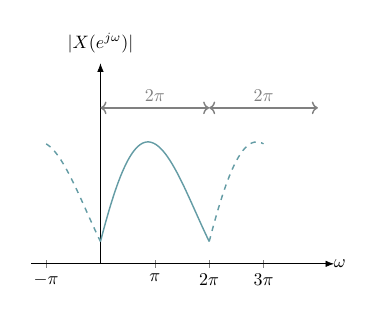
\begin{tikzpicture}[scale=0.65]
                \begin{axis}[
                    width=7.5cm, height=5.5cm,
                    axis lines=middle, axis line style={-{Latex}},
                    xmin=-4, xmax=13.5, ymin=0, ymax=1.8,
                    xtick={-3.14, 0, 3.14, 6.28, 9.42}, xticklabels={$-\pi$, $0$, $\pi$, $2\pi$, $3\pi$},
                    ytick=\empty,
                    xlabel={$\omega$}, ylabel={$|X(e^{j\omega})|$},
                    clip=false,
                    ylabel style={yshift=20pt, anchor=north},
                    xlabel style={xshift=10pt, anchor=east},
                    declare function={
                            dtftbase(\x) = 1.2*abs(sin(deg(\x/2)))*exp(-0.1*\x) + 0.2;
                            dtft(\x) = (\x < 0) ? dtftbase(\x + 6.283) : ((\x > 6.283) ? dtftbase(\x - 6.283) : dtftbase(\x));
                        }
                    ]
                    \addplot[samples=150, domain=0:6.28, thick, AccentColor] {dtft(x)};
                    \addplot[samples=100, domain=-3.14:0, thick, AccentColor, dashed] {dtft(x)};
                    \addplot[samples=100, domain=6.28:9.42, thick, AccentColor, dashed] {dtft(x)};

                    \draw[<->, thick, gray] (axis cs:0,1.4) -- node[above] {$2\pi$} (axis cs:6.28,1.4);
                    \draw[<->, thick, gray] (axis cs:6.28,1.4) -- node[above] {$2\pi$} (axis cs:12.56,1.4); % Just an arrow pointing right
                \end{axis}
            \end{tikzpicture}
        \end{center}
    \end{minipage}
\end{frame}

\begin{frame}{DFT as a Sampled DTFT}
    \begin{minipage}{0.5\textwidth}
        \begin{itemize}

            \item Comparing $X(e^{j\omega})$ with,
                  \begin{align*}
                      X[k] = \sum_{n=0}^{N-1} x[n]e^{-j\frac{2\pi}{N}kn}
                  \end{align*}
                  We see that the DFT evaluates $X(e^{j\omega})$ exactly at evenly spaced discrete frequencies $\omega_k = \frac{2\pi}{N}k$:
                  \begin{equation*}
                      X[k] = X(e^{j\omega})\Big|_{\omega = \frac{2\pi}{N}k}
                  \end{equation*}
            \item Thus, the $N$-point DFT is simply $N$ equispaced samples of the continuous DTFT exactly over one $2\pi$ period.
        \end{itemize}
    \end{minipage}
    \hfill
    \begin{minipage}{0.48\textwidth}
        \begin{center}
            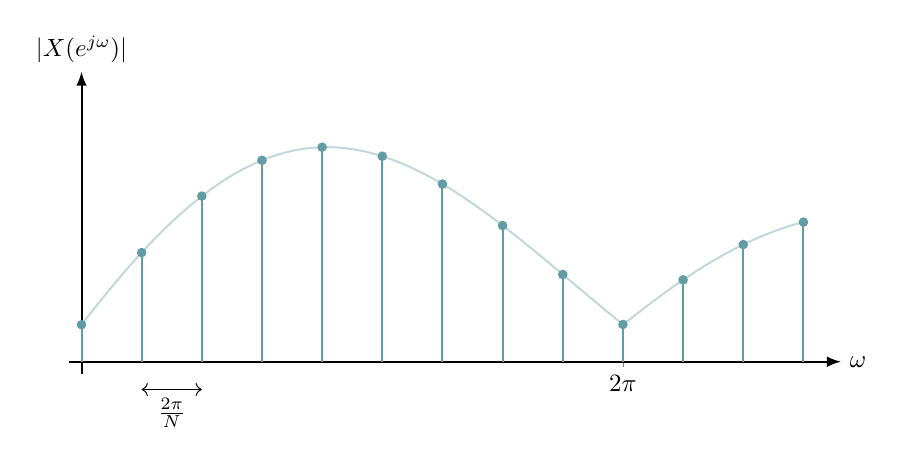
\begin{tikzpicture}[scale=0.9]
                \begin{axis}[
                    width=\textwidth, height=5.5cm,
                    axis lines=middle, axis line style={shorten >=-5pt, shorten <=-5pt, -{Latex[length=2mm]}, thick},
                    xmin=0, xmax=6.5, ymin=0, ymax=1.5,
                    xtick={0, 4.71}, xticklabels={0, $2\pi$},
                    ytick=\empty,
                    xlabel={$\omega$}, ylabel={$|X(e^{j\omega})|$},
                    xlabel style={anchor=west,xshift=5pt}, ylabel style={anchor=south,yshift=5pt},
                    clip=false,
                    declare function={dtft(\x) = 1.2*abs(sin(deg(\x/1.5)))*exp(-0.1*\x) + 0.2;}
                    ]
                    \addplot[name path=f, samples=100, domain=0:6.28, thick, AccentColor!40] {dtft(x)};
                    \addplot[ycomb, mark=*, mark size=1.5pt, thick, AccentColor, samples=13, domain=0:6.28] {dtft(x)};
                    \draw[<->] (axis cs:0.523,-0.15) -- node[below] {$\frac{2\pi}{N}$} (axis cs:1.047,-0.15);
                \end{axis}
            \end{tikzpicture}
        \end{center}
    \end{minipage}
\end{frame}

\begin{frame}{Zero-Padding for Increased Frequency Resolution}
    \begin{minipage}{0.48\textwidth}
        \begin{itemize}
            \item \textbf{Zero-Padding}: For an aperiodic $x[n]$ of length $N$, we can artificially append zeros to define it over a total length $M \ge N$.
            \item Taking the $M$-point DFT samples the \textit{same} continuous DTFT spectrum $X(e^{j\omega})$, but at a much finer resolution of \textbf{$2\pi/M$}!
        \end{itemize}
    \end{minipage}
    \hfill
    \begin{minipage}{0.48\textwidth}
        \begin{center}
            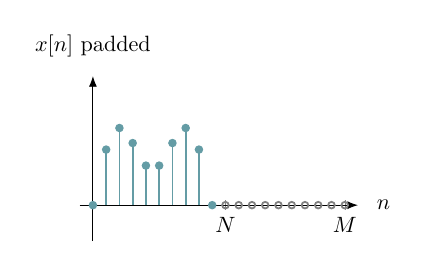
\begin{tikzpicture}[scale=0.8]
                \begin{axis}[
                    name=ax1,
                    width=6cm, height=4.2cm,
                    axis lines=middle, axis line style={-{Latex}},
                    xmin=-1, xmax=20, ymin=-0.5, ymax=1.8,
                    xtick={10, 19}, xticklabels={$N$, $M$},
                    ytick=\empty, xlabel={$n$}, ylabel={$x[n]$ padded}, clip=false,
                    xlabel style={anchor=west,xshift=5pt}, ylabel style={anchor=south,yshift=5pt},
                    declare function={sig(\t) = (\t>=0 && \t<=9) ? (sin(deg(pi*\t/9)) + 0.5*sin(deg(3*pi*\t/9))) : 0;}
                    ]
                    \addplot[ycomb, mark=*, mark size=1.5pt, thick, AccentColor, samples=10, domain=0:9] {sig(x)};
                    \addplot[ycomb, mark=o, mark size=1.5pt, thick, gray, samples=10, domain=10:19] {0};
                \end{axis}
            \end{tikzpicture}

            \vspace{0.5cm}

            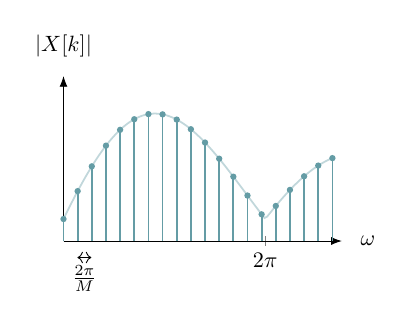
\begin{tikzpicture}[scale=0.8]
                \begin{axis}[
                    name=ax2,
                    width=6cm, height=4.2cm,
                    axis lines=middle, axis line style={-{Latex}},
                    xmin=0, xmax=6.5, ymin=0, ymax=1.5,
                    xtick={0, 4.71}, xticklabels={0, $2\pi$},
                    ytick=\empty, xlabel={$\omega$}, ylabel={$|X[k]|$}, clip=false,
                    xlabel style={anchor=west,xshift=5pt}, ylabel style={anchor=south,yshift=5pt},
                    declare function={dtft(\x) = 1.2*abs(sin(deg(\x/1.5)))*exp(-0.1*\x) + 0.2;}
                    ]
                    \addplot[name path=f, samples=100, domain=0:6.28, thick, AccentColor!40] {dtft(x)};
                    % Finer samples M=24 instead of N=12
                    \addplot[ycomb, mark=*, mark size=1pt, thick, AccentColor, samples=20, domain=0:6.28] {dtft(x)};
                    \draw[<->] (axis cs:0.325,-0.15) -- node[below] {$\frac{2\pi}{M}$} (axis cs:0.65,-0.15);
                \end{axis}
            \end{tikzpicture}
        \end{center}
    \end{minipage}
\end{frame}

\end{document}
